%%%%%%%%%%%%  Generated using docx2latex.com  %%%%%%%%%%%%%%

%%%%%%%%%%%%  v2.0.0-beta  %%%%%%%%%%%%%%

\documentclass[12pt]{article}
\usepackage{amsmath}
\usepackage{latexsym}
\usepackage{amsfonts}
\usepackage[normalem]{ulem}
\usepackage{soul}
\usepackage{array}
\usepackage{amssymb}
\usepackage{extarrows}
\usepackage{graphicx}
\usepackage[backend=biber,
style=numeric,
sorting=none,
isbn=false,
doi=false,
url=false,
]{biblatex}\addbibresource{bibliography.bib}

\usepackage{subfig}
\usepackage{wrapfig}
\usepackage{wasysym}
\usepackage{enumitem}
\usepackage{adjustbox}
\usepackage{ragged2e}
\usepackage[svgnames,table]{xcolor}
\usepackage{tikz}
\usepackage{longtable}
\usepackage{changepage}
\usepackage{setspace}
\usepackage{hhline}
\usepackage{multicol}
\usepackage{tabto}
\usepackage{float}
\usepackage{multirow}
\usepackage{makecell}
\usepackage{fancyhdr}
\usepackage[toc,page]{appendix}
\usepackage[hidelinks]{hyperref}
\usetikzlibrary{shapes.symbols,shapes.geometric,shadows,arrows.meta}
\tikzset{>={Latex[width=1.5mm,length=2mm]}}
\usepackage{flowchart}\usepackage[paperheight=11.69in,paperwidth=8.27in,left=1.18in,right=1.18in,top=0.98in,bottom=0.98in,headheight=1in]{geometry}
\usepackage[utf8]{inputenc}
\usepackage[T1]{fontenc}
\TabPositions{0.49in,0.98in,1.47in,1.96in,2.45in,2.94in,3.43in,3.92in,4.41in,4.9in,5.39in,5.88in,}

\urlstyle{same}

\renewcommand{\_}{\kern-1.5pt\textunderscore\kern-1.5pt}

 %%%%%%%%%%%%  Set Depths for Sections  %%%%%%%%%%%%%%

% 1) Section
% 1.1) SubSection
% 1.1.1) SubSubSection
% 1.1.1.1) Paragraph
% 1.1.1.1.1) Subparagraph


\setcounter{tocdepth}{5}
\setcounter{secnumdepth}{5}


 %%%%%%%%%%%%  Set Depths for Nested Lists created by \begin{enumerate}  %%%%%%%%%%%%%%


\setlistdepth{9}
\renewlist{enumerate}{enumerate}{9}
		\setlist[enumerate,1]{label=\arabic*)}
		\setlist[enumerate,2]{label=\alph*)}
		\setlist[enumerate,3]{label=(\roman*)}
		\setlist[enumerate,4]{label=(\arabic*)}
		\setlist[enumerate,5]{label=(\Alph*)}
		\setlist[enumerate,6]{label=(\Roman*)}
		\setlist[enumerate,7]{label=\arabic*}
		\setlist[enumerate,8]{label=\alph*}
		\setlist[enumerate,9]{label=\roman*}

\renewlist{itemize}{itemize}{9}
		\setlist[itemize]{label=$\cdot$}
		\setlist[itemize,1]{label=\textbullet}
		\setlist[itemize,2]{label=$\circ$}
		\setlist[itemize,3]{label=$\ast$}
		\setlist[itemize,4]{label=$\dagger$}
		\setlist[itemize,5]{label=$\triangleright$}
		\setlist[itemize,6]{label=$\bigstar$}
		\setlist[itemize,7]{label=$\blacklozenge$}
		\setlist[itemize,8]{label=$\prime$}

\setlength{\topsep}{0pt}\setlength{\parskip}{8.04pt}
\setlength{\parindent}{0pt}

 %%%%%%%%%%%%  This sets linespacing (verticle gap between Lines) Default=1 %%%%%%%%%%%%%%


\renewcommand{\arraystretch}{1.3}


%%%%%%%%%%%%%%%%%%%% Document code starts here %%%%%%%%%%%%%%%%%%%%



\begin{document}


%%%%%%%%%%%%%%%%%%%% Figure/Image No: 1 starts here %%%%%%%%%%%%%%%%%%%%

\begin{figure}[H]
	\begin{Center}
		
\includegraphics[width=1.92in,height=2.24in]{./media/image1.pdf}
	\end{Center}
\end{figure}


%%%%%%%%%%%%%%%%%%%% Figure/Image No: 1 Ends here %%%%%%%%%%%%%%%%%%%%

\setlength{\parskip}{0.0pt}
\par


\vspace{\baselineskip}
\setlength{\parskip}{8.04pt}
\begin{Center}
{\fontsize{18pt}{21.6pt}\selectfont \textbf{UNIVERSIDADE FEDERAL DA FRONTEIRA SUL}\par}
\end{Center}\par


\vspace{\baselineskip}

\vspace{\baselineskip}

\vspace{\baselineskip}
\begin{Center}
{\fontsize{24pt}{28.8pt}\selectfont \textbf{CONJUNTOS NUMÉRICOS}\par}
\end{Center}\par


\vspace{\baselineskip}
\begin{Center}
{\fontsize{16pt}{19.2pt}\selectfont Professores:\par}
\end{Center}\par

\begin{Center}
{\fontsize{20pt}{24.0pt}\selectfont \textbf{Pedro Augusto Pereira Borges}\par}
\end{Center}\par


\vspace{\baselineskip}

\vspace{\baselineskip}

\vspace{\baselineskip}
\begin{Center}
{\fontsize{14pt}{16.8pt}\selectfont Colaborador:\par}
\end{Center}\par

\begin{Center}
{\fontsize{20pt}{24.0pt}\selectfont \textbf{Fernando Augusto Brancher}\par}
\end{Center}\par


\vspace{\baselineskip}

\vspace{\baselineskip}
\begin{Center}
\textbf{FEVEREIRO/2015}
\end{Center}\par



 %%%%%%%%%%%%  Starting New Page here %%%%%%%%%%%%%%

\newpage

\vspace{\baselineskip}\setlength{\parskip}{0.0pt}
\begin{enumerate}[label*=\arabic*.]
	\item \textbf{Introdução\  }
\end{enumerate}\par

A criação dos números, como conhecemos hoje, é produto da evolução de ideias sobre como representar determinadas grandezas, resolver problemas geométricos, problemas aplicados às ciências e resolução de equações. \par

A noção de número inteiro foi criada pela necessidade de contar objetos, animais e pessoas. Nossos antepassados contavam somente até dois, a partir disto, o conjunto de coisas era dado como $``$muitos$"$  (BOYER, p.2). Alguns índios, até hoje, têm dificuldades em contar até três (KARLSON, p.5). Inicialmente o homem contava com os dedos, com grãos, com pequenas pedras ou fazendo marcas em bastões, relacionando a eles os objetos de seu interesse: uma pedra, um búfalo; uma família, os dedos de uma mão. É a contagem por correspondência um a um.\par

Cada cultura desenvolveu uma representação simbólica. Os egípcios, antes de 5.000 a.C. usavam um sistema de numeração com barras e figuras para resolver problemas bem mais complexos do que a simples contagem. Os romanos criaram um sistema de representação com letras, mas com limitações para efetuar operações. Os hindus, por volta de 595 d.C. usavam nove símbolos, e dois séculos depois, incluíram o zero, completando um sistema de numeração posicional, com algoritmos eficientes para operações, que os árabes divu/lgaram pela Europa, mais tarde. \par

Problemas de comércio e contabilidade motivaram o uso de sinais em números para representar ganhos e perdas. Diofanto já operava com negativos, no século III. \par

Os povos antigos (egípcios, mesopotâmios, hindus e chineses) enunciaram e resolveram problemas algébricos e geométricos, cujas soluções era não inteira, evidenciando o conhecimento e uso de números fracionários. Os pitagóricos (século V a.C.) não conseguiram explicar a natureza do número que representa a medida da diagonal de um quadrado e com isso geraram a necessidade de criar números não racionais. \par

Durante o século XIX e século XX o movimento de axiomatização da matemática levou à construção dos conjuntos numéricos, com base na teoria dos conjuntos. Tal construção foi desenvolvida por Giuseppe Peano. \par

O conhecimento sobre a natureza dos números é importante para as ciências puras e aplicadas, apesar do senso comum reduzir as aplicações a números inteiros ou fracionários (no sentido de não inteiro). O número de funcionários de uma empresa, de carros, de pizzas, de sapatos, de vacas, ..., são quantidades inteiras. Não se pode considerar meio funcionário, meio carro ou meia vaca. O tempo, os valores monetários, o número de toneladas (massa) de arroz, soja, feijão, ..., são variáveis fracionárias. Trabalhamos com meia hora, com meio dólar, etc. Porém, o comprimento da hipotenusa de uma tesoura triangular de telhado pode ser aproximado por um número fracionário finito, mas é um número irracional, para a grande maioria dos casos. Da mesma forma, grandezas da eletricidade requerem a definição de números não reais, chamados de complexos. Assim, para entendermos as expressões matemáticas das variáveis, com clareza e precisão, precisamos conhecer os tipos de números, suas propriedades e operações.\par


\vspace{\baselineskip}
\begin{adjustwidth}{0.37in}{0.0in}
\textbf{2. Conjunto dos Números Naturais ( \( N \) )}\par

\end{adjustwidth}

A contagem de quantidades inteiras de animais, pessoas ou coisas, foi provavelmente, o que motivou a criação dos números naturais.\par

\tab  \( N \) \textit{ = $ \{ $ 0,1,2,3,4,...$ \} $ }\par

O conjunto dos números naturais é infinito e pode ser representado em uma reta numerada com pontos cheios:\par



%%%%%%%%%%%%%%%%%%%% Figure/Image No: 2 starts here %%%%%%%%%%%%%%%%%%%%

\begin{figure}[H]
	\begin{Center}
		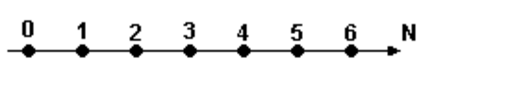
\includegraphics[width=3.44in,height=0.58in]{./media/image2.pdf}
	\end{Center}
\end{figure}


%%%%%%%%%%%%%%%%%%%% Figure/Image No: 2 Ends here %%%%%%%%%%%%%%%%%%%%

\par

Os intervalos no conjunto dos números naturais são escritos usando os símbolos \par

> maior \par

< menor \par

 maior ou igual e\par

 menor ou igual.\par

Vejamos os exemplos:\par

\begin{adjustwidth}{0.89in}{0.0in}
\textbf{Exemplo 2.1 – Escreva os elementos do conjunto  A=$ \{ $ \textit{x   \( N \)  / x > 2$ \} $  (Lê-se: x pertence aos Naturais, tal que x é maior do que 2) e represente-os em uma reta.}}\par

\end{adjustwidth}

\begin{adjustwidth}{0.89in}{0.0in}
\textbf{Solução: Escrevendo os elementos de A, temos: A=$ \{ $ \textit{3,4,5,6,7,...$ \} $ .}}\par

\end{adjustwidth}

\begin{adjustwidth}{0.63in}{0.0in}
Mostrando esse conjunto na reta dos números naturais, colocamos pontos cheios pretos para os elementos do conjunto \textbf{A e vazios para os elementos que não pertencem ao conjunto A.}\par

\end{adjustwidth}



%%%%%%%%%%%%%%%%%%%% Figure/Image No: 3 starts here %%%%%%%%%%%%%%%%%%%%

\begin{figure}[H]
	\begin{Center}
		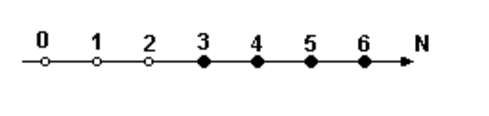
\includegraphics[width=3.26in,height=0.77in]{./media/image3.pdf}
	\end{Center}
\end{figure}


%%%%%%%%%%%%%%%%%%%% Figure/Image No: 3 Ends here %%%%%%%%%%%%%%%%%%%%

\par

\begin{adjustwidth}{0.63in}{0.0in}
\textbf{Exemplo 2.2 - Escreva os elementos do conjunto\  B=$ \{ $ \textit{x   \( N \)  / 1< x <5$ \} $  ( Lê-se: x pertence aos Naturais, tal que x é maior do que 1 e menor do que 5. (ou, x pertence aos Naturais , tal que 1 é menor do que x e x é menor do que 5) e represente-os em uma reta.}}\par

\end{adjustwidth}

\begin{adjustwidth}{0.63in}{0.0in}
\textbf{Solução: Usando a mesma representação do Exemplo 2.1, temos: B=$ \{ $ \textit{2,3,4$ \} $ . Mostrando esse conjunto na reta dos números naturais, temos:}}\par

\end{adjustwidth}



%%%%%%%%%%%%%%%%%%%% Figure/Image No: 4 starts here %%%%%%%%%%%%%%%%%%%%

\begin{figure}[H]
	\begin{Center}
		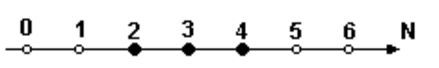
\includegraphics[width=2.93in,height=0.45in]{./media/image4.pdf}
	\end{Center}
\end{figure}


%%%%%%%%%%%%%%%%%%%% Figure/Image No: 4 Ends here %%%%%%%%%%%%%%%%%%%%

\tab \par

\begin{adjustwidth}{0.63in}{0.0in}
\textbf{Exemplo 2.3 – Escreva os elementos do conjunto C, representado na reta numerada:}\par

\end{adjustwidth}



%%%%%%%%%%%%%%%%%%%% Figure/Image No: 5 starts here %%%%%%%%%%%%%%%%%%%%

\begin{figure}[H]
	\begin{Center}
		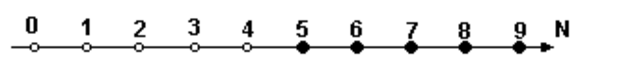
\includegraphics[width=4.17in,height=0.51in]{./media/image5.pdf}
	\end{Center}
\end{figure}


%%%%%%%%%%%%%%%%%%%% Figure/Image No: 5 Ends here %%%%%%%%%%%%%%%%%%%%

\tab \par

\begin{adjustwidth}{0.63in}{0.0in}
\textbf{Solução:\tab Podemos escrever os elementos desse conjunto de duas maneiras: por extensão (descrevendo um a um) }\par

\end{adjustwidth}

\begin{adjustwidth}{0.63in}{0.0in}
\tab  \textbf{C=$ \{ $ \textit{5,6,7,8,9,10,...$ \} $  }}\par

\end{adjustwidth}

\begin{adjustwidth}{0.63in}{0.0in}
\tab ou usando os símbolos de desigualdade  \par

\end{adjustwidth}

\begin{adjustwidth}{0.63in}{0.0in}
\  \tab \textbf{C=$ \{ $ \textit{x   \( N \)  / x  5$ \} $ \ \ \ ou\ ainda   C=$ \{ $ x   \( N \)  / x  4$ \} $ \ \ \ \  ■}}\par

\end{adjustwidth}

\tab 
\vspace{\baselineskip}\textbf{EXERCÍCIOS 2}\par

\begin{enumerate}
	\item Escreva por extensão os elementos dos conjuntos:\par

a)\  \textbf{A=$ \{ $ \textit{x   \( N \)  / x > 5$ \} $ \tab \tab \tab d)\  D=$ \{ $ x   \( N \)  / 2  x < 8$ \} $ }}\par

b)\  \textbf{B=$ \{ $ \textit{x   \( N \)  / 1 < x < 10$ \} $ \tab \tab e)\  E=$ \{ $ x   \( N \)  / 2 < x  5$ \} $ }}\par

c)\  \textbf{C=$ \{ $ \textit{x   \( N \)  / x  6$ \} $ \tab \tab \tab f)  F=$ \{ $ x   \( N \)  / 2 > x ou x > 5$ \} $ }}\par

	\item Represente os conjuntos do Ex.1 graficamente.\par

	\item Verifique se as quantidades das grandezas abaixo podem ser expressas com números naturais:\par

a) População de uma cidade.\par

b) Número de porcos criados em uma granja por ano.\par

c) A velocidade de uma pessoa em uma corrida de maratona.\par

d) O número de escovas de dentes produzido mensalmente por uma indústria.\par

e) A taxa de variação da cesta básica em um estado do Brasil em um determinado mês.\par

	\item As notas das provas escolares são expressas em números naturais?\par

	\item Existe um número \textbf{natural} X que somado com 5 dê 3? (ou seja: 5 + X = 3)\par

	\item Verifique se as operações abaixo geram números naturais:
\end{enumerate}\par

\begin{adjustwidth}{0.2in}{0.0in}
a) 5 + 8 = \tab \tab \tab c) 5 $ \cdot $ \  8 = \par

\end{adjustwidth}

\begin{adjustwidth}{0.2in}{0.0in}
b) 3 – 5 =\tab \tab \tab \tab d) 8 : 5 =\par

\end{adjustwidth}


\vspace{\baselineskip}
\begin{enumerate}
	\item \textbf{Conjunto dos Números Inteiros Relativos ( \( Z \) )}
\end{enumerate}\par

As letras (b) e (d) do Exercício 1.1.6 ilustram problemas de operações com números naturais cuja solução gera números não naturais. Portanto, é necessário admitir a existência de outros tipos de números.\par

Se as quantidades ou grandezas inteiras mudam seu significado de acordo com um referencial, pode-se representa-las usando um sinal e um número. Vejamos alguns exemplos:\par

\textbf{Saldo bancário: se temos dinheiro depositado, dizemos que o saldo é positivo. Se gastamos mais dinheiro do que temos e o banco nos empresta, dizemos que o saldo é negativo. Assim, se o saldo é +3.500,00 reais, significa que temos esse montante na conta. A referência, é o saldo zero. Neste caso, não temos nada, mas também não devemos ao banco.}\par

\textbf{Temperatura: a temperatura é uma grandeza associada ao estado térmico de um corpo: Quanto mais calor o corpo possui, maior será a temperatura e quanto mais frio, menor. Pela escala Celsius, a referência é a temperatura da água congelada: \textit{0 \textsuperscript{oC. Assim, na madrugada de um dia de inverno podemos ter temperaturas negativas, como -5oC e ao meio-dia, positivas, como + 15oC.}}}\par

\textbf{Taxas de variações: as variações de cotação de moedas, como o dólar, por exemplo, são dadas usando a referência zero, ou seja quando não varia. Assim, \textit{+2 $\%$  significa que o dólar subiu em relação à última cotação; ou -2 $\%$  significa que o dólar 'caiu'. Essas taxas de variações são muito usadas na economia: na bolsa de valores para indicar a tendência das ações; nas análises de desempenho de empresas (crescimento/decrescimento). Na física, o sinal da velocidade de um corpo indica o sentido do deslocamento. }}\par

Os números inteiros relativos podem ser representados da seguinte forma: \par

 \( Z \)  =$ \{ $ \textit{...,-6,-5,-4-3,-2,-1,0,+1,+2,+3,+4,+5,+6,...$ \} $ }\par

A representação gráfica do conjunto  \( Z \)  é:\par



%%%%%%%%%%%%%%%%%%%% Figure/Image No: 6 starts here %%%%%%%%%%%%%%%%%%%%

\begin{figure}[H]
	\begin{Center}
		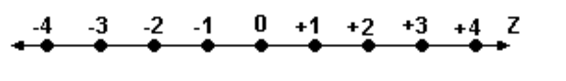
\includegraphics[width=3.77in,height=0.54in]{./media/image6.pdf}
	\end{Center}
\end{figure}


%%%%%%%%%%%%%%%%%%%% Figure/Image No: 6 Ends here %%%%%%%%%%%%%%%%%%%%

\par

Escrevendo o conjunto  \( Z \)  usando símbolos, temos: \par

 \( Z \)  =$ \{ $ \textit{ x   \( Z \)  / - < x < +$ \} $ .}\par


\vspace{\baselineskip}
\textbf{3.1 - Operações em  \( Z \) }\par

\textbf{Adição e subtração de números inteiros}\par


\vspace{\baselineskip}
Ao operar com números inteiros relativos, precisamos identificar inicialmente a \textbf{\textit{operação solicitada e em seguida o sinal dos números.}}\par



%%%%%%%%%%%%%%%%%%%% Figure/Image No: 7 starts here %%%%%%%%%%%%%%%%%%%%

\begin{figure}[H]
	\begin{Center}
		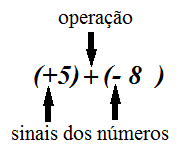
\includegraphics[width=1.88in,height=1.64in]{./media/image7.png}
	\end{Center}
\end{figure}


%%%%%%%%%%%%%%%%%%%% Figure/Image No: 7 Ends here %%%%%%%%%%%%%%%%%%%%

\par

\par 
 \begin{tikzpicture}

\path (3.11in,-0.92in) node [shape=rectangle,draw,minimum height=1.53in,minimum width=5.46in,]{};
{\fontsize{14pt}{16.8pt}\selectfont \textbf{Regra da adição de dois números inteiros\par}: }
\path (2.75in,-0.31in) node [shape=single arrow,draw,minimum height=0.24in,minimum width=0.85in,]{};
\tab sinais iguais \tab \tab \tab \tab \textbf{adiciona e usa o mesmo sinal no \tab \tab \tab \tab \tab \tab \tab \tab \tab \tab \tab resultado}
\path (2.76in,-0.31in) node [shape=single arrow,draw,minimum height=0.24in,minimum width=0.85in,]{};
\tab sinais diferentes\tab \tab \tab \textbf{subtrai e usa o sinal do maior no \tab \tab \tab \tab \tab \tab \tab \tab \tab \tab \tab resultado}
\end{tikzpicture}

\vspace{\baselineskip}
\textbf{Exemplos:}\par

1)\textbf{ \  \textit{(+5) + (+3) = +5+3 = +8\tab \tab \tab 3)\  (-5) + (+ 3) = -5 + 3 = -2}}\par

2)\ \  \textit{(+5) + (- 3) = +5 - 3 = +2 \tab \tab 4)\  (-5) + (- 3) = -5 - 3 = -8\tab }\par


\vspace{\baselineskip}
\textbf{Multiplicação e divisão de números inteiros}\par

\par 
 \begin{tikzpicture}

\path (3.06in,-0.47in) node [shape=rectangle,draw,minimum height=0.76in,minimum width=5.29in,]{};
{\fontsize{14pt}{16.8pt}\selectfont \textbf{Regra da Subtração de dois números inteiros}:\par}
\end{tikzpicture}
Troca\ o sinal do segundo número e usa a regra da adição.  \par


\vspace{\baselineskip}
\textbf{Exemplos:}\par

1)\textbf{\ \   \textit{(+5) - (+ 3) = (+5) + (- 3) = +2\tab \tab 3)\ \  (-5) - (- 3) = (-5) + (+ 3) = - 2}}\par

2)\ \  \textit{(+5) - (- 3) = (+5) + (+ 3) = +8\tab \tab 4)\ \  (-5) - (+ 3) = (-5) + (- 3) = - 8}\par


\vspace{\baselineskip}

\vspace{\baselineskip}
\par 
 \begin{tikzpicture}

\path (2.98in,-0.61in) node [shape=rectangle,draw,minimum height=1.22in,minimum width=5.21in,]{};
{\fontsize{14pt}{16.8pt}\selectfont \textbf{Regra da Multiplicação e Divisão: }(para o sinal do resultado)\par}
\path (2.71in,-0.35in) node [shape=single arrow,draw,minimum height=0.24in,minimum width=0.85in,]{};
\tab sinais iguais\tab \tab \tab  \tab resultado positivo
\path (2.7in,-0.32in) node [shape=single arrow,draw,minimum height=0.24in,minimum width=0.85in,]{};
\tab sinais diferentes \tab \tab \tab  resultado negativo
\end{tikzpicture}

\vspace{\baselineskip}
\textbf{Exemplos:\ \ \  }\par

\setlength{\parskip}{6.0pt}
\begin{enumerate}
	\item \textit{(+5) $ \cdot $  (+4) = +20\tab \tab \tab 3)\  (+20) : (+4) = +5}\par

	\item \textit{(+20) : (-4) = - 5\tab \tab \tab 4) (+5) $ \cdot $  (-4) = - 20\tab \tab }\par


\vspace{\baselineskip}
\setlength{\parskip}{0.0pt}
\textbf{Potênciação de números inteiros}\par

\par 
 \begin{tikzpicture}

\path (2.86in,-1.3in) node [shape=rectangle,draw,minimum height=1.9in,minimum width=5.71in,]{};

\end{tikzpicture}
\setlength{\parskip}{8.04pt}
\textbf{Definição 3.1: }A potência\  \textit{b\textsuperscript{n}}\  , para  o expoente \textit{n $ \epsilon $   \( N \) } e a base \textit{b $ \epsilon $   \( Z \) \  ,} é o produto de \textit{b}, \textit{n} vezes, por ele mesmo:\par



%%%%%%%%%%%%%%%%%%%% Figure/Image No: 8 starts here %%%%%%%%%%%%%%%%%%%%

\begin{figure}[H]
	\begin{Center}
		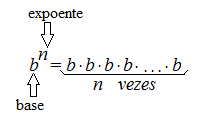
\includegraphics[width=2.05in,height=1.2in]{./media/image8.png}
	\end{Center}
\end{figure}


%%%%%%%%%%%%%%%%%%%% Figure/Image No: 8 Ends here %%%%%%%%%%%%%%%%%%%%

\setlength{\parskip}{0.0pt}
\tab \tab \tab \tab \par


\vspace{\baselineskip}
\setlength{\parskip}{8.04pt}
\textbf{Exemplos: }Calcule \ \  (a) \textit{2\textsuperscript{4}} , (b) (-3)\textit{\textsuperscript{3} , } (c) (\textit{-2)\textsuperscript{4}} e (d) \textit{-2\textsuperscript{4}}\par

\textbf{Solução}: \par

(a) \textit{2\textsuperscript{4}}\ =\ 2 $ \cdot $  2 $ \cdot $  2  $ \cdot $  2  = \textit{16}\par

(b) (-3)\textit{\textsuperscript{3}\  = (-3)} $ \cdot $  \textit{(-3)} $ \cdot $  \textit{(-3)} = \textit{-27}\par

(c) \textit{(-2)\textsuperscript{4} = (-2)} $ \cdot $  \textit{(-2)} $ \cdot $  \textit{(-2)} $ \cdot $  \textit{(-2)=\ 16  }\par

(d) -2\textit{\textsuperscript{4}\  = -2 }$ \cdot $  \textit{2} $ \cdot $  \textit{2} $ \cdot $ \textit{2 = -16}\par

\par 
 \begin{tikzpicture}

\path (2.7in,-1.15in) node [shape=rectangle,draw,minimum height=2.16in,minimum width=5.56in,]{};
\setlength{\parskip}{0.0pt}
\textbf{Observemos que:}
\end{tikzpicture}
\begin{enumerate}
	\item Se a base é positiva (\textit{b > 0}) então \textit{b\textsuperscript{n}}\  > 0.\par

	\item Se a base é negativa (\textit{b < 0}) e :\par

\tab Se \textit{n é par então b\textsuperscript{n\  > 0}}\par

\tab Se \textit{n é ímpar então b\textsuperscript{n\  < 0.}}\par

	\item Se a base é 1 (\textit{b = 1}) então \textit{b\textsuperscript{n}}\  \textit{= 1}, para qualquer \textit{n $ \epsilon $   \( N \) .} 
\end{enumerate}\par


\vspace{\baselineskip}
\setlength{\parskip}{8.04pt}

\vspace{\baselineskip}
\setlength{\parskip}{0.0pt}
\textbf{Radiciação de números inteiros}\par


\vspace{\baselineskip}
\par 
 \begin{tikzpicture}

\path (3.09in,-0.49in) node [shape=rectangle,draw,minimum height=0.97in,minimum width=5.78in,]{};
\setlength{\parskip}{8.04pt}
\begin{adjustwidth}{1.28in}{0.0in}
\textbf{Definição 3.2: }A raiz\  \textit{n-ézima, }para\textit{ n }  \( N \)  , de um número \textit{b}   \( Z \) \  é \textit{x}   \( Z \)  se e somente se \textit{x\textsuperscript{n} = b}.\  \end{adjustwidth}


\end{tikzpicture}

\vspace{\baselineskip}
\begin{adjustwidth}{1.28in}{0.0in}
 \[ \sqrt[n]{b}=x~~ \Longleftrightarrow   x^{n}=b. \] \par

\end{adjustwidth}


\vspace{\baselineskip}
\textbf{Exemplos}:\par

\begin{enumerate}
	\item  \( \sqrt[3]{8}=2~~ \Longleftrightarrow   2^{3}=8. \) \par

	\item  \( \sqrt[3]{ \left( -8 \right) }=-2~~ \Longleftrightarrow    \left( -2 \right) ^{3}=-8. \) \par

	\item  \( \sqrt[]{10}~~ \) não é um número inteiro, pois \textit{3\textsuperscript{2} < 10 < 4\textsuperscript{2}}.\par

	\item  \( \sqrt[]{4}=-2~~ \Longleftrightarrow    \left( -2 \right) ^{2}=4 \) ,\ mas também   \( \sqrt[]{4}=2~~ \Longleftrightarrow    \left( 2 \right) ^{2}=4 \) . 
\end{enumerate}\par

\begin{adjustwidth}{1.23in}{0.0in}
Então\   \( \sqrt[]{4}= \pm ~2   \) ■\par

\end{adjustwidth}


\vspace{\baselineskip}
\setlength{\parskip}{0.0pt}
\textbf{EXERCÍCOS 3}\par

	\item Resolva as expressões numéricas:\par

a)\tab \textit{(+15)+(-12) =\tab \tab \tab b) (-15)+(-10) =}\par

c)\tab \textit{(+8)+(-12)-(+5) =\tab \tab \tab d) (-7)-(-9)-(+3) =}\par

e)\tab \textit{(+6) : (-3) =\tab \tab \tab \tab f) (-7)  (-5) =}\par

g)\tab \textit{1- (-3)+(-4)=\tab \tab \tab h) -4-[3+5(5 - 2)]=}\par

i) \tab \textit{3(5 - 8)-(8 - 3)+6=\tab \tab \tab j) -[-4 -3(7-4)-(2-5)]=}\par

	\item \colorbox{Red}{O saldo bancário de um correntista no dia 1\textsuperscript{o }do mês era de R$\$$  3.500,00 e no dia 3, entrou um cheque para ser descontado de R$\$$  4.350,00. Qual é o saldo no dia 3 ? }\par

	\item Expresse e resolva as seguintes situações, usando números relativos:\par

\tab a) Uma pessoa tem \textit{50 reais e \textbf{perde 30 reais.}}\par

\tab b) Uma pessoa tem \textit{100 reais e \textbf{paga uma dívida 40.}}\par

\tab c) Uma pessoa tem uma \textbf{dívida de \textit{100 reais e ganha 50 reais.}}\par

\tab d) Uma pessoa tem uma \textbf{dívida de \textit{200 reais e perde 70 reais.}}\par

	\item Em um dia de inverno a temperatura máxima foi de \textit{18\textsuperscript{o}C} e a mínima de \textit{-3\textsuperscript{o}C} . Qual foi a variação de temperatura?\par

	\item Uma peça de metal estava a \textit{80\textsuperscript{o}C }e foi resfriada variando sua temperatura em\textit{ \tab 90\textsuperscript{o}C. }Qual é a temperatura final da peça?\par

	\item Considere o nível do mar como altitude \textit{0 m}, acima positiva e abaixo negativa. Se a cidade \textbf{A} está a \textit{+ 450 m} e a \textbf{B} está a \textit{+230 m}, qual é a diferença de altitude \tab entre as cidades?\par

	\item Existe um número \textbf{inteiro} X que somado com 5 dê 3? (ou seja: 5 + X = 3)\par

	\item A divisão\  6/2\ \ é  número \textbf{inteiro} ? e a divisão 6/4 ?\par

	\item Resolva as potências:\par

\setlength{\parskip}{8.04pt}
\begin{enumerate}
	\item \textit{4\textsuperscript{2}} \tab \tab c) 0\textsuperscript{5} \tab \tab e)  \(  \left( -5 \right) ^{2} \) \tab \tab g)  \( -2^{4} \) \par

	\item (-4)\textsuperscript{3\tab }\tab d) 1\textsuperscript{100} \tab \tab f)  \(  \left( -2 \right) ^{4} \) \tab \tab h)  \( -2^{5} \) 
\end{enumerate}\par

\setlength{\parskip}{0.0pt}
	\item  Resolva as raízes:
\end{enumerate}\par

\begin{enumerate}
	\item  \( \sqrt[]{9} \)  \tab \tab c)  \( \sqrt[3]{-27} \)  \tab e)  \( \sqrt[6]{64} \)  \tab g)  \( \sqrt[5]{-32} \) \par

	\item  \( \sqrt[3]{27} \)  \tab \tab d)  \( \sqrt[4]{16} \) \tab \tab f)  \( \sqrt[5]{32} \) \tab \tab h)  \( \sqrt[3]{-64} \) \  
\end{enumerate}\par


\vspace{\baselineskip}
\begin{justify}
\textbf{4 - Conjunto dos Números Racionais ( \( Q \) )}
\end{justify}\par

\begin{justify}
Os números racionais são aqueles que podem ser escritos na forma de fração  \( \frac{a}{b} \) , onde \textit{a} e \textit{b} são números inteiros, com \textit{b} diferente de zero. Simbolizamos o conjunto dos racionais com a letra \textbf{\textit{Q}}\textit{ .} Escrevendo em linguagem matemática:
\end{justify}\par

 \( Q \)  = $ \{ $ \textit{ x   \( Q \) \textbf{  se x = a/b $ \} $  para a e b  \( ~Z \)  e b $ \neq $  0.}}\par

\begin{justify}
Assim, qualquer fração é um número racional, por exemplo  \( \frac{1}{2} \)  ;  \( \frac{5}{4} \)  ; \( -\frac{3}{5} \) ; ...
\end{justify}\par

\begin{justify}
Da mesma forma, qualquer número inteiro é também um número racional, pois podemos escrevê-lo em forma de fração. Por exemplo:
\end{justify}\par

\begin{justify}
 \( 2=\frac{4}{2}=\frac{10}{5} \) ;\ \ \ \ \ \ \ \ \ \ \ \ \   \( -5=\frac{-10}{2}=\frac{30}{-6}=-\frac{15}{3} \) .
\end{justify}\par

\textbf{Equivalência de frações}: uma fração  \( \frac{a}{b} \)   não se altera se multiplicamos ou dividimos o numerador e o denominador pelo mesmo número \textit{m}, desde que\textit{ m $ \neq $  0 }e\textit{ m   \( Z \) }.\par

 \tab \tab {\fontsize{14pt}{16.8pt}\selectfont   \( \frac{a}{b}=\frac{a \cdot m}{b \cdot m} \) \ \ \ \ \ \  ou\ \ \ \ \ \   \( \frac{a}{b}=\frac{\text{a~ : m}}{\text{b~ : m}} \)  \par}\par

\begin{justify}
Observe-se que para a divisão, \textit{a} e \textit{b} devem ser divisíveis por \textit{m}. Com essa propriedade podemos transformar uma fração em outra equivalente, porém com denominador diferente. Vejamos os exemplos:
\end{justify}\par

\textbf{Exemplos:}\par

\begin{enumerate}
	\item  \( \frac{1}{2}=\frac{2}{4} \)  . Nesse caso, a primeira fração foi multiplicada por \textit{m=2}.\par


\vspace{\baselineskip}
	\item   \( \frac{12}{8}=\frac{3}{2} \) {\fontsize{16pt}{19.2pt}\selectfont  . Esse caso é conhecido como simplificação de frações. Dividimos o numerador e o denominador por \textit{m=4.} \par}\par


\vspace{\baselineskip}
\setlength{\parskip}{8.04pt}
\setlength{\parskip}{0.0pt}
	\item Para\ transformar   \( \frac{3}{4} \) \  em uma fração com denominador igual 16, podemos usar \textit{m=4}.\ Assim\    \( \frac{3}{4}=\frac{12}{16} \) \  são equivalentes.
\end{enumerate}\par


\vspace{\baselineskip}
\textbf{4.1 - Adição e subtração de frações }\par

\tab O sinal do resultado da adição e subtração de frações segue as regras operatórias dos números inteiros e das operações com frações.\par

\tab 
\vspace{\baselineskip}\tab \textbf{Frações com denominadores iguais:}\par

Sejam \textit{a, b} e \textit{c} números inteiros: \par

\textbf{\tab \ \ \ \   \( \frac{a}{b}+\frac{c}{b}=\frac{a+c}{b} \) \tab }{\fontsize{16pt}{19.2pt}\selectfont \tab , para \textit{b \   \( Z \)  $ \neq $  0}.\par}\par

\textbf{Exemplos: }\par

\begin{enumerate}
	\item  \( \frac{1}{4}+\frac{5}{4}=\frac{1+5}{4}=\frac{6}{4}=\frac{3}{2} \) \tab \tab b)  \( \frac{3}{5}-\frac{4}{5}=\frac{3-4}{5}=\frac{-1}{5}=-\frac{1}{5} \) \tab 
\end{enumerate}\par


\vspace{\baselineskip}
\tab \textbf{Frações com denominadores diferentes}: \par

\begin{justify}
Se os denominadores das frações são diferentes, transformamos as frações de tal forma que os denominadores sejam iguais. Usar o menor múltiplo comum (MMC) dos denominadores das frações dadas como denominador das novas frações é uma estratégia bem eficiente. Ou de modo geral, 
\end{justify}\par

\begin{justify}
\  \tab \tab  \( \frac{a}{b}+\frac{c}{d}=\frac{ad+cb}{bd}~~~ \) {\fontsize{16pt}{19.2pt}\selectfont  , para \textit{b }e\textit{ d  \   \( Z \)   $ \neq $  0} ■\par}
\end{justify}\par

\textbf{Exemplos:}\par

\begin{enumerate}
	\item  \( \frac{1}{4}+\frac{3}{2}=\frac{1+6}{4}=\frac{7}{4} \) \tab \tab \tab 2){\fontsize{16pt}{19.2pt}\selectfont   \( \frac{1}{4}-\frac{2}{3}=\frac{3-8}{12}=-\frac{5}{12} \) \par}
\end{enumerate}\par


\vspace{\baselineskip}
\textbf{4.2 - Multiplicação de frações:}\par

Sejam \textit{a, b,c} e \textit{d} números inteiros: \par


\vspace{\baselineskip}
\par 
 \begin{tikzpicture}

\path (2.78in,-0.58in) node [shape=rectangle,draw,minimum height=0.95in,minimum width=5.72in,]{};
\textbf{Multiplica-se numerador com numerador e denominador com denominador. }
\end{tikzpicture}
\setlength{\parskip}{6.0pt}
\tab \tab \tab  \( \frac{a}{b} \cdot \frac{c}{d}=\frac{a  \cdot c }{b  \cdot d} \) \tab \tab , para \textit{b} e \textit{d} \textit{\   \( Z \) } $ \neq $  0.\par


\vspace{\baselineskip}
\setlength{\parskip}{0.0pt}
\tab \textbf{Exemplos:}\par

\begin{enumerate}
	\item  \( \frac{1}{4} \cdot \frac{3}{2}=\frac{3}{8} \) \tab \tab \tab 2){\fontsize{16pt}{19.2pt}\selectfont   \( \frac{1}{4} \cdot  \left( -\frac{2}{3} \right) =-\frac{2}{12}=-\frac{1}{6} \) \par}
\end{enumerate}\par


\vspace{\baselineskip}
\textbf{Propriedade do cancelamento:}\par

Algumas multiplicações podem ser simplificadas, diminuindo os números a serem operados.\par

\textbf{Exemplos: }\par

1)\ Resolva\ \    \( \frac{12}{5} \cdot \frac{3}{2}\text{~~~ .} \) \par

Simplificando o \textit{12} com o \textit{2}, por \textit{2,} obtemos   \( \frac{6}{5} \cdot \frac{3}{1}=\frac{18}{5} \) {\fontsize{16pt}{19.2pt}\selectfont .\par}\par

2) Resolva\textbf{  \( \frac{18}{15} \cdot \frac{5}{2} \cdot \frac{9}{2}\text{~~~ .} \) }\par

\begin{adjustwidth}{0.2in}{0.0in}
\begin{justify}
A utilização da regra da multiplicação diretamente, neste caso, gera operações com números relativamente grandes. Utilizando o cancelamento, essa dificuldade é remediada.
\end{justify}\par

\end{adjustwidth}

Simplificando o \textit{18} com \textit{2} e o \textit{15} com o \textit{5}, obtemos  \( \frac{9}{3} \cdot \frac{1}{1} \cdot \frac{9}{2}. \) \par

Simplificando o \textit{3} com o \textit{9}, obtemos  \( \frac{3}{1} \cdot \frac{1}{1} \cdot \frac{9}{2}=\frac{27}{2}~. \) \tab \par


\vspace{\baselineskip}
\textbf{4.3 - Divisão de frações}\par


\vspace{\baselineskip}
\par 
 \begin{tikzpicture}

\path (2.86in,-0.55in) node [shape=rectangle,draw,minimum height=1.07in,minimum width=5.01in,]{};
\setlength{\parskip}{12.0pt}
\tab Inverte-se a segunda fração e multiplica-se pela primeira.
\end{tikzpicture}
\  \tab \tab  \( \frac{a}{b}:\frac{c}{d}=\frac{a}{b} \cdot \frac{d}{c}=\frac{ad}{bc}~~ \) \  , para \textit{b} e \textit{d} \textit{\   \( Z \) }  $ \neq $   0.\par

\setlength{\parskip}{0.0pt}
\begin{adjustwidth}{0.49in}{0.0in}
A regra dos sinais é idêntica à regra da divisão dos números inteiros.\par

\end{adjustwidth}


\vspace{\baselineskip}
\tab \textbf{Demonstração: }\par


\vspace{\baselineskip}
Seja \   \( \frac{a}{b}~:~\frac{c}{d}=N \) , sendo \textit{N} \textit{\   \( Q \) .}\par

\setlength{\parskip}{8.04pt}
\begin{adjustwidth}{0.2in}{0.0in}
Escrevendo\ \   \( \frac{a}{b}~:~\frac{c}{d}=N \) \  como  \( ~~\frac{~\frac{a}{b}}{\frac{c}{d}}~ =N \)  , pode-se multiplicar ambos os membros dessa equação por \textit{d/c}.\par

\end{adjustwidth}

\tab  \( ~~\frac{~\frac{a}{b}}{\frac{c}{d}}  \cdot  \frac{c}{d} =N  \cdot  \frac{c}{d} \) \par

Cancelando o denominador \textit{c/d}\  com o fator \textit{c/d}\  do primeiro membro, tem-se:\par

\tab  \( ~\frac{a}{b}~ =N  \cdot  \frac{c}{d} \) \par

Para isolar \textit{N}, multiplica-se ambos os membros dessa equação por \textit{d/c}. Tem-se:\par

\tab  \( \frac{a}{b} \cdot  \frac{d}{c}~ =N  \cdot  \frac{c}{d} \cdot  \frac{d}{c}=N \) \par


\vspace{\baselineskip}
O produto das frações do lado direito é 1. Portanto, tem-se:\par

\tab  \( N=\frac{a}{b}~:~\frac{c}{d}= \frac{a}{b} \cdot  \frac{d}{c} =\frac{ad}{bc}~ \) \ \ \  ■\tab \par

\setlength{\parskip}{0.0pt}
\textbf{Exemplos:}\par

\begin{enumerate}
	\item  \( \frac{3}{4}:\frac{1}{2}=\frac{3}{4} \cdot \frac{2}{1}=\frac{3}{2} \) \tab \tab 2){\fontsize{16pt}{19.2pt}\selectfont   \(  \left( -\frac{1}{3} \right) : \left( -\frac{2}{5} \right) = \left( -\frac{1}{3} \right)  \cdot  \left( -\frac{5}{2} \right) =+\frac{5}{6} \) \par}
\end{enumerate}\par


\vspace{\baselineskip}
\textbf{4.4 – Números decimais e frações }\par

Os \textit{números decimais finitos} podem ser representados na forma de frações decimais, usando a propriedade da equivalência de frações. Portanto, são números racionais. Veja os exemplos:\par

\textbf{Exemplos:}\par

1)  \( 0,3=0,3 \cdot \frac{10}{10}=\frac{3}{10}~~ \) \tab \tab \tab \tab \par

2)  \( 0,25=0,25 \cdot \frac{100}{100}=\frac{25}{100}~~ \)  \tab \tab \tab \tab \par

3)  \( 1,302=1,302 \cdot \frac{1000}{1000}=\frac{1302}{1000}~~ \) \ \ \ \  \par


\vspace{\baselineskip}
\begin{justify}
Generalizando a ideia apresentada nestes exemplos, podemos afirmar que para representar um número decimal finito na forma de fração
\end{justify}\par


\vspace{\baselineskip}
\par 
 \begin{tikzpicture}


% Error occured here... ignoring it.
\begin{Center}
\textbf{Escrevemos o número sem a vírgula sobre \textit{10$ \cdot $ n}, sendo \textit{n} o número de casas depois da vírgula do número decimal.}
\end{Center}
\end{tikzpicture}

\vspace{\baselineskip}
\begin{justify}
Os números \textit{decimais periódicos infinitos} também podem ser representados na forma de frações. Veja os exemplos:
\end{justify}\par


\vspace{\baselineskip}
\begin{justify}
\textbf{Exemplo 1} – Represente a dízima periódica 0,33333.... na forma de fração.
\end{justify}\par

\begin{justify}
\textbf{Solução: }Vamos chamar esse número de \textit{r}:
\end{justify}\par

\begin{adjustwidth}{0.69in}{0.0in}
\begin{justify}
\tab \textit{r = 0,333333....} . Multiplicando a equação toda por \textit{10}, porque o período tem somente um algarismo, temos:
\end{justify}\par

\end{adjustwidth}

\begin{adjustwidth}{0.69in}{0.0in}
\begin{justify}
\tab \textit{10r = 3,33333....} . Re-escrevendo o lado direito da igualdade, temos:
\end{justify}\par

\end{adjustwidth}

\begin{adjustwidth}{0.69in}{0.0in}
\begin{justify}
\tab \textit{10r = 3 + 0,33333.... = 3 + r} .\ \  Adicionando (-r) nos dois lados da equação, temos:
\end{justify}\par

\end{adjustwidth}

\begin{adjustwidth}{0.69in}{0.0in}
\begin{justify}
\tab \textit{10r – r = 3}
\end{justify}\par

\end{adjustwidth}

\begin{adjustwidth}{0.69in}{0.0in}
\begin{justify}
\tab \textit{9r = 3}
\end{justify}\par

\end{adjustwidth}

\begin{adjustwidth}{0.69in}{0.0in}
\begin{justify}
\tab  \( r=\frac{3}{9}=\frac{1}{3}~~ \) \textit{, }portanto 1/3 é um número racional\textit{ ■}
\end{justify}\par

\end{adjustwidth}

\tab 
\vspace{\baselineskip}\begin{justify}
\textbf{Exemplo 2} – Represente a dízima periódica \textit{r = 0,12121212....} na forma de fração.
\end{justify}\par

\begin{justify}
\textbf{Solução: }Multiplicando a equação toda por \textit{100}, porque o período tem dois algarismos, temos:
\end{justify}\par

\tab \tab 
\vspace{\baselineskip}\tab \textit{100 r = 12,121212 $ \ldots $ } . Re-escrevendo o lado direito da igualdade, temos:\tab \par

\tab \textit{100 r = 12 + 0,12121212... = 12 + r}.\  Adicionando (\textit{-r}) nos dois lados da equação, temos:\par

\tab \textit{100r – r = 12}\par

\textit{\tab 99r = 12}\par

\tab  \( r=\frac{12}{99}~~~ \) \textit{\ \ \  ,} portanto 12/99 é um número racional\textit{■}\par


\vspace{\baselineskip}
\tab Regra para escrever dízimas periódicas, menores do que 1, na forma de fração:\par

\par 
 \begin{tikzpicture}

\path (3.2in,-0.6in) node [shape=rectangle,draw,minimum height=0.92in,minimum width=5.56in,]{};
\begin{adjustwidth}{0.49in}{0.0in}
\begin{justify}
\textbf{1º\   Escreve-se os algarismos do período no numerador;}
\end{justify}\end{adjustwidth}


\end{tikzpicture}
\begin{adjustwidth}{0.49in}{0.0in}
\begin{justify}
\textbf{2º\   Escreve-se o denominador com tantos noves, quantos forem os algarismos do período.}
\end{justify}\par

\end{adjustwidth}


\vspace{\baselineskip}
\tab Com esta regra, podemos representar qualquer dízima periódica na forma de um número racional. Veja os exemplos e confira com sua calculadora:\par

\textbf{Exemplos:}\par

1)  \( 0,2222 \ldots =\frac{2}{9} \)  \tab \tab 2)  \( 0,252525 \ldots =\frac{25}{99} \) \tab \tab 3)\   \( 0,245245245 \ldots =\frac{245}{999} \) \par

\begin{adjustwidth}{0.25in}{0.0in}
\textbf{EXERCÍCIOS 4}\par

\end{adjustwidth}


\vspace{\baselineskip}
\begin{enumerate}
	\item Resolva as adições e subtrações com as frações:\par

a)\textbf{  \(  \left( -\frac{1}{3} \right) + \left( -\frac{2}{3} \right) = \) \tab \tab \tab }d){\fontsize{16pt}{19.2pt}\selectfont   \( -\frac{2}{7}-\frac{3}{14}+\frac{3}{2}= \) \par}\par

b){\fontsize{16pt}{19.2pt}\selectfont   \(  \left( -\frac{4}{3} \right) - \left( -\frac{2}{5} \right) + \left( -\frac{1}{6} \right) = \) \tab e)  \( -\frac{5}{6}+\frac{3}{8}+\frac{1}{2}= \) \par}\par

c)  \( 1+\frac{3}{10}-\frac{12}{15}= \) \tab \tab \tab f){\fontsize{16pt}{19.2pt}\selectfont   \( ~\frac{5}{2}-2+\frac{2}{4}= \) \par}\par


\vspace{\baselineskip}
	\item Resolva as operações com as expressões fracionárias:
\end{enumerate}\par

\begin{adjustwidth}{0.25in}{0.0in}
a)\textbf{  \( \frac{1}{2}- \left( \frac{1}{3}+\frac{2}{3} \right) =~  \) \tab \tab \tab }d)\textbf{  \( -3 \cdot  \left( -\frac{1}{3}+\frac{2}{5} \right) =~  \) \tab }\par

\end{adjustwidth}

\begin{adjustwidth}{0.25in}{0.0in}
b)\   \( -\frac{1}{3} \cdot  \left( -2+\frac{2}{3} \right) =~  \) \ \ \ \ \ \ \  \tab \tab e)\   \( -5: \left( \frac{1}{2}-\frac{2}{3} \right) =~~  \) \par

\end{adjustwidth}

\begin{adjustwidth}{0.25in}{0.0in}
c)  \( -6 \cdot  \left( \frac{1}{3}+\frac{3}{4} \right) =~  \) \tab \tab \tab f)\ \   \( -3 \cdot  \left( -\frac{1}{3} \right) +\frac{3}{4}:\frac{3}{2}=~  \) \ \ \ \ \ \ \  \par

\end{adjustwidth}


\vspace{\baselineskip}

\vspace{\baselineskip}

\vspace{\baselineskip}
\begin{enumerate}[label*={\fontsize{12pt}{12pt}\selectfont \textbf{\arabic*.}}]
	\item \textbf{- Conjunto dos números reais ()}\par

Os recursos utilizados para escrever uma dízima periódica na forma de fração, tem por base o fato de existir um período (números que se repetem). Existem muitos números decimais não periódicos. Vejamos alguns exemplos:\par

\textit{$ \pi $  = 3,1415926....... Conhecido como número pi. Está presente em vários problemas de geometria.}\par

\textit{e = 2,7182818284590452353602874... Conhecido como número de Euler, ou número e.}\par

 \( \sqrt[]{2}=1,414214 \ldots  \)  É uma raiz não exata. As raízes não exatas não são dízimas periódicas.\par

\textit{ø =1,6180339887... ou \   \(  \varnothing =\frac{1+\sqrt[]{5}}{2} \) \  é conhecido como o número de ouro, amplamente usado por arquitetos gregos para projetar construções e por artistas para determinar proporções em desenhos do corpo humano. }\par

A esses números, \textit{que é impossível escreve-los na forma de fração, damos o nome de números irracionais. Além de números especiais como o pi, o número de Euler e o número de ouro, as raízes não exatas são exemplos mais comuns de números irracionais. O uso das propriedades e operações com raízes não exatas (radicais) são frequentes em aplicações na ciência.}\par

\textbf{Definição 5.1 - O conjunto dos Números Reais é a união do conjunto dos Racionais e dos Irracionais. }\par

\tab  \( R \)  =  \( Q \)   \textbf{\textit{I\ \ \  ■}}\par


\vspace{\baselineskip}
A representação do conjunto  \( R \)  na reta numérica é uma reta cheia (reta real).\par



%%%%%%%%%%%%%%%%%%%% Figure/Image No: 9 starts here %%%%%%%%%%%%%%%%%%%%

\begin{figure}[H]
	\begin{Center}
		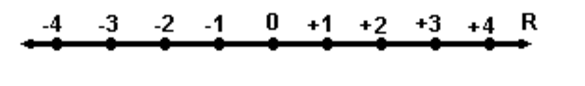
\includegraphics[width=3.9in,height=0.57in]{./media/image9.pdf}
	\end{Center}
\end{figure}


%%%%%%%%%%%%%%%%%%%% Figure/Image No: 9 Ends here %%%%%%%%%%%%%%%%%%%%

\par

Veja alguns exemplos de intervalos em  \( R \) \textbf{ e suas respectivas representações na reta numerada:}\par



%%%%%%%%%%%%%%%%%%%% Figure/Image No: 10 starts here %%%%%%%%%%%%%%%%%%%%

\begin{figure}[H]
	\begin{Center}
		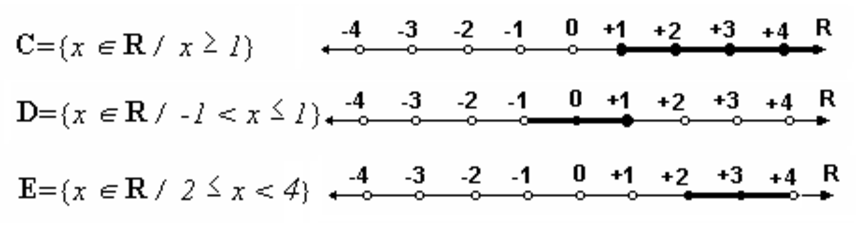
\includegraphics[width=5.72in,height=1.53in]{./media/image10.pdf}
	\end{Center}
\end{figure}


%%%%%%%%%%%%%%%%%%%% Figure/Image No: 10 Ends here %%%%%%%%%%%%%%%%%%%%

\par

Os conjuntos também podem ser representados usando parêntesis para \textit{intervalos abertos, por exemplo:}\par

(a,b) significa $ \{ $ \textit{ x   \( R \)  / a < x < b$ \} $ }\par

e com colchetes para \textit{intervalos fechados, por exemplo:}\par

[a,b] significa =$ \{ $ \textit{ x   \( R \)  / a  x  b$ \} $ .}\par


\vspace{\baselineskip}
\textbf{Definição 5.2: Seja\  \textit{b um número real,\  m e n\ números inteiros positivos.  Então,}}\par


\vspace{\baselineskip}
\tab   \( b^{\frac{m}{n}}=\sqrt[n]{b^{m}} \) {\fontsize{14pt}{16.8pt}\selectfont .\par}\par

\textbf{Exemplo: \( ~~\sqrt[3]{3^{2}}=3^{\frac{2}{3}} \) \  ■}\par


\vspace{\baselineskip}
\begin{enumerate}[label*=\textbf{\arabic*.}]
	\item \textbf{Propriedades dos radicais}
\end{enumerate}
\end{enumerate}\par

Sejam \textit{a e b números reais; m,n e p números inteiros positivos maiores do que 1.}\par

\textbf{P1)  \( \sqrt[n]{a \cdot b}=\sqrt[n]{a} \cdot \sqrt[n]{b} \) }\par

\textbf{P2)  \( \sqrt[n]{\frac{a}{b}}=\frac{\sqrt[n]{a}}{\sqrt[n]{b}} \) \ \ para  \textit{b $ \neq $ \  0.}}\par

\textbf{P3)  \( \sqrt[n]{\sqrt[m]{b}}=\sqrt[nm]{b} \) }\par

\textbf{P4)  \(  \left( \sqrt[n]{b^{m}} \right) ^{p}=\sqrt[n]{a^{mp}} \) }\par

\textbf{P5) Para b $ \geq $ \ 0    \( \sqrt[n]{b^{n}}=b . \) }\par

\textbf{P6)\ Para\ b\ <\ 0       \( \sqrt[n]{b^{n}}= \left\{ \begin{matrix}
 \vert b \vert  se n é par\\
-b se n é ímpar\\
\end{matrix}
 ~ \) }\par


\vspace{\baselineskip}
\textbf{Exemplos: Simplifique os radicais:}\par

\begin{enumerate}
	\item  \( \sqrt[3]{81} \)  . Para simplificar esse radical vamos utilizar as propriedades P1 e P5.\par

 \[ \sqrt[3]{81}=\sqrt[3]{3^{4}}=\sqrt[3]{3^{3} \cdot 3}=3 \cdot \sqrt[3]{3} \] \par

	\item  \( \sqrt[]{27y^{9}} \) \ \  se y > 0. Para simplificar esse radical vamos utilizar as propriedades P1 e P5.
\end{enumerate}\par

\tab  \( \sqrt[]{27y^{9}}=\sqrt[]{3  \cdot 3^{2} \cdot y^{8} \cdot y}=3y^{4}\sqrt[]{\text{3 y}} \) \  ■\tab \tab \par

\textbf{5.2 - Racionalização de denominadores}\par

O denominador de algumas frações podem ter radicais. Nesse caso podemos usar a propriedade P5 para racionalizar (tornar racional) o denominador. \par

\begin{adjustwidth}{0.5in}{0.0in}
\textbf{Exemplo: Racionalize o denominador da fração\ \    \( \frac{1}{\sqrt[]{3}}. \) }\par

\end{adjustwidth}

\begin{adjustwidth}{0.5in}{0.0in}
\textbf{Solução: Multiplicando-se a fração dada por 1, escrito na forma  \( \frac{\sqrt[]{3}}{\sqrt[]{3}}. \) \ \  não a alteramos. Então,  \( \frac{1}{\sqrt[]{3}} \cdot \frac{\sqrt[]{3}}{\sqrt[]{3}}=\frac{\sqrt[]{3}}{3} \) \  ■}\par

\end{adjustwidth}


\vspace{\baselineskip}
\textbf{5.3 - Operações com radicais}\par

\begin{enumerate}
	\item \textbf{Adição e subtração}:
\end{enumerate}\par

\begin{adjustwidth}{0.74in}{0.0in}
Só é possível adicionar ou subtrair radicais semelhantes (\textit{índices e radicandos idênticos). }\par

\end{adjustwidth}

\begin{adjustwidth}{0.74in}{0.0in}
\textbf{Exemplos:}\par

\end{adjustwidth}

\begin{enumerate}
	\item  \( \sqrt[]{2}+3\sqrt[]{2}-5\sqrt[]{2}=-\sqrt[]{2} \) \par

	\item  \( \sqrt[]{3}-2\sqrt[]{27}-\frac{\sqrt[]{12}}{2}.~ \)  Nesse caso, os radicais não são semelhantes. Porém,\par

 \( \sqrt[]{27}=3\sqrt[]{3} \) \ \ e   \( \frac{\sqrt[]{12}}{2}=\frac{2\sqrt[]{3}}{2}=\sqrt[]{3} \) \ \  (usando as propriedades \textbf{P1 e P5). Substituindo estas igualdades na expressão dada, temos:}\par

 \( \sqrt[]{3}-3\sqrt[]{3}-\sqrt[]{3}=-3\sqrt[]{3}~ \) .\par

	\item Multiplicação e divisão de radicais:
\end{enumerate}\par

\begin{adjustwidth}{0.99in}{0.0in}
As propriedades \textbf{P1 e P2 resolvem as operações de multiplicação e divisão, respectivamente, para radicais de mesmo índice. }\par

\end{adjustwidth}

\begin{adjustwidth}{0.79in}{0.0in}
\textbf{Exemplos:}\par

\end{adjustwidth}

\begin{enumerate}
	\item  \( \sqrt[]{2} \cdot \sqrt[]{5}=\sqrt[]{10} \) \  . Foi usada a propriedade P1.\par

	\item  \( \sqrt[]{6}\text{~ : }\sqrt[]{2}=\sqrt[]{3} \) \ \ \  Foi usada a propriedade P2.\par

	\item  \( \sqrt[]{3} \cdot \sqrt[4]{2}= \) \par

Como o MMC(2,4)=4,\ vamos transformar os radicais equivalentes com índice  4 e usar a propriedade P1.\par

 \[ \sqrt[2 \cdot 2]{3^{1 \cdot 2}} \cdot \sqrt[4]{2}=\sqrt[4]{3^{2}} \cdot \sqrt[4]{2}=\sqrt[4]{18} \] \par

	\item  \( \sqrt[4]{2} \cdot \sqrt[6]{3}= \) \par

Como o MMC(4,6)=12,\ vamos transformar os radicais equivalentes com índice  12 e usar a propriedade P1.\par

 \[ \sqrt[4 \cdot 3]{2^{1 \cdot 3}} \cdot \sqrt[6 \cdot 2]{3^{1 \cdot 2}}=\sqrt[12]{8} \cdot \sqrt[12]{9}=\sqrt[12]{72} \] \par

	\item  \( \sqrt[4]{2} \cdot \sqrt[6]{2}= \) 
\end{enumerate}\par

\begin{adjustwidth}{0.59in}{0.0in}
Como o MMC(4,6)=12,\ vamos transformar os radicais equivalentes com índice  12 e usar a propriedade P1..\par

\end{adjustwidth}

\begin{adjustwidth}{0.59in}{0.0in}
 \[ \sqrt[4 \cdot 3]{2^{1 \cdot 3}} \cdot \sqrt[6 \cdot 2]{2^{1 \cdot 2}}=\sqrt[12]{2^{5}}= \] \par

\end{adjustwidth}

\begin{adjustwidth}{0.59in}{0.0in}
Nesse caso (bases dos radicandos iguais) poderíamos usar a Def. 1.4.2 e resolver como multiplicação de potências de mesmas bases.\par

\end{adjustwidth}

\begin{adjustwidth}{0.59in}{0.0in}
 \( \sqrt[4]{2} \cdot \sqrt[6]{2}=2^{\frac{1}{4}} \cdot 2^{\frac{1}{6}}=2^{\frac{5}{12}}=\sqrt[12]{2^{5}}~~~~~ \) ■\par

\end{adjustwidth}


\vspace{\baselineskip}
\begin{adjustwidth}{0.99in}{0.0in}
\textbf{EXERCÍCIOS 5}\par

\end{adjustwidth}

\begin{enumerate}
	\item Calcule as raízes:\par

\begin{enumerate}
	\item  \( \sqrt[3]{27} \) \tab \ \ \ \  b)  \( \sqrt[3]{\frac{8}{27}} \) \tab \ \ \  c)  \( \sqrt[3]{64} \) \tab d)  \( \sqrt[5]{32} \) \ \ \ \ \ \ \ \ \  e)  \( \frac{\sqrt[]{64}}{\sqrt[4]{16}} \) \ \ \ \ \ \ \ \ \ \ \  f)  \( \sqrt[4]{\frac{625}{81}} \) \tab 
\end{enumerate}\par

	\item Os radicais do Ex.5.1 são números racionais ou irracionais?\par

	\item Simplifique os radicais:\par

 \( a \right)  \sqrt[]{8} \) \tab \ \  b)  \( \sqrt[]{12} \) \tab c)  \( \sqrt[3]{24} \) \tab \tab  d)  \( \sqrt[4]{32} \) \ \ \ \ \ \ \ \  e)  \( \sqrt[]{\frac{12}{45}} \) \ \ \ \ \ \  \tab f)  \( \sqrt[3]{\frac{16}{125}} \) \tab \par

	\item Os radicais do Ex 5.3 são números racionais ou irracionais?\par

	\item Coloque os coeficientes no radicando:\par

\tab  \( a \right)  2\sqrt[]{3} \) \tab \ \ \ \  b)  \( 3\sqrt[3]{2} \) \tab c)  \( 7\sqrt[]{2} \) \tab d)  \( \frac{1}{2}\sqrt[3]{4} \) \ \ \ \ \ \  e)  \( 3~ \cdot   \sqrt[]{\frac{1}{2}} \) \tab \ \ \ \ \ \ \ \  f)  \( 5~ \cdot   \sqrt[]{\frac{3}{4}} \) \par

	\item Resolva as operações com os radicais:\par

a)  \( 3\sqrt[]{3}+5\sqrt[]{3}-\sqrt[]{3} \) \  \tab \ \ \  b)  \( \sqrt[]{\frac{1}{2}}-~3  \sqrt[]{\frac{1}{2}} \) \tab \ \  c)  \( \sqrt[]{5}  \cdot  \sqrt[3]{2} \) \tab \ \ \ \ \  d)  \( \sqrt[]{3}  \cdot  \sqrt[]{5} \cdot \sqrt[]{\frac{1}{2}} \)  e)  \( \sqrt[3]{\frac{3}{4}} \cdot 3~ \sqrt[3]{\frac{1}{2}} \) \ \ \ \  \tab \ \ \ \ \ \  f)  \( ~7\sqrt[]{5}  \cdot  3\sqrt[]{2} \) \ \ \ \ \ \ \ \ \ \ \ \  g)  \( \sqrt[]{10}~:~\sqrt[]{2} \) \ \ \ \ \ \ \ \ \ \ \ \  h)  \( \sqrt[]{10}\text{~ : }\sqrt[]{\frac{1}{2}} \) \par

	\item Resolva os produtos:
\end{enumerate}\par

\begin{enumerate}
	\item  \( 2~ \left( \sqrt[]{5}+3\sqrt[]{5} \right)  \) \tab \tab \tab b)  \( \sqrt[]{2}~ \left( \sqrt[]{3}+\sqrt[]{5} \right)  \) \tab \tab c)  \( \sqrt[]{6}~ \left( \sqrt[]{32}-\sqrt[]{3} \right)  \) \ \  d)  \(  \left( 2+\sqrt[]{2} \right)  \cdot  \left( 2-\sqrt[]{2} \right)  \) \ \ \ \  \tab e)\   \(  \left( 3-\sqrt[]{5} \right) ^{2} \) \ \ \ \ \ \ \  f)  \(  \left( \sqrt[]{7}-2\sqrt[]{3} \right)  \cdot  \left( \sqrt[]{7}+2\sqrt[]{3} \right)  \) \tab \tab 
\end{enumerate}\par

\begin{adjustwidth}{0.3in}{0.0in}
\textbf{5.8\tab  Racionalize os denominadores:}\par

\end{adjustwidth}

\begin{enumerate}
	\item  \( \frac{1}{\sqrt[]{3}} \) \tab \ \ \  b)  \( \frac{3}{\sqrt[]{2}} \) \tab \  c)  \( \frac{7}{\sqrt[]{5}} \) \tab \ \ \ \ \  \tab d)  \( \frac{3}{2+\sqrt[]{3}} \) \tab \tab e)  \( \frac{1}{\sqrt[]{2}-\sqrt[]{3}} \) \tab \colorbox{Red}{f)  \( \frac{35}{\sqrt[]{3}-5} \) }
\end{enumerate}\par

\textbf{5.9\ \ \  Verifique\ se\ \ \    \( \frac{-3}{2}=\frac{3}{-2}=-\frac{3}{2~} \) .}\par

\textbf{5.10 Escreva o respectivo conjunto numérico a que pertence cada um dos seguintes números:  0; $-$ 1; $-$ 34;  \( \sqrt[3]{8} \) ; 0,454545...; 212; $-$ 46;  \( \sqrt[3]{2} \) ; 12,1829421; 2,99999... e 3,76.}\par

\textbf{5.11 Explique porque \textit{-5 é um número inteiro e também é um número racional.}}\par

\textbf{5.12 Explique porque \textit{$-$ 15 é um número racional e também é um número inteiro.}}\par

\textbf{5.13 Escreva os números abaixo em forma de fração:}\par

\begin{adjustwidth}{0.3in}{0.0in}
\tab a) \textit{0, 3}= \tab \tab \tab b) \textit{0, 55555.}..=\tab \tab \tab c) \textit{1, 32}= \tab \tab \par

\end{adjustwidth}

\begin{adjustwidth}{0.3in}{0.0in}
\tab \colorbox{Red}{d) \textit{0, 212121}...=\tab \tab e) \textit{1, 3333..}.=} \tab \tab \tab f) \textit{3, 434343}...=\par

\end{adjustwidth}


\vspace{\baselineskip}
\begin{enumerate}[label*={\fontsize{12pt}{12pt}\selectfont \arabic*.}]
	\item  Explique porque \textit{0, 77777...} é um número racional.\par


\vspace{\baselineskip}
	\item  Explique porque \  $ \pi $  = 3, 1415927... é um número irracional.\par


\vspace{\baselineskip}
	\item  Explique porque  \( \frac{4}{6}=\frac{2}{3} \)  \ \  \par


\vspace{\baselineskip}
\setlength{\parskip}{8.04pt}
\setlength{\parskip}{6.0pt}
	\item  Indique o conjunto de números adequado para cada variável:\par

\tab a) Tempo de vida de um pé de milho\par

\tab b) Altura de um pé de soja\par

\tab c) Número de vacas de uma propriedade\par

\tab d) Produção leiteira\par

\tab e) Teor de água do solo.\par

\tab f) Massa de solo.\par

\tab g) Massa de um suíno.\par

\tab h) Volume de água de uma amostra de solo.\par

\tab i) Número de frangos em um aviário.\par

\tab j) Diagonal de um quadrado.\par

	\item  Escreva os intervalos por compreensão:\par

\tab a) \textbf{\textit{A}}\textit{=$ \{ $ 1,2,3,4,5$ \} $ } \tab \tab \tab \tab \tab b) \textbf{\textit{B}}\textit{=$ \{ $ -3,-2,-1,0,1,2$ \} $ }\par

\tab c) os números reais maiores ou iguais a -3 \tab d) os números reais entre -3 e 5\par

\tab e) os números reais menores que 3 e maiores que 5\par

	\item  Represente os intervalos na reta real:\par

\tab a) \textbf{\textit{P}}\textit{ = $ \{ $ x $ \epsilon $  \textbf{R }/ $-$  1 < x < 3$ \} $ } \tab \tab b) \textbf{\textit{K}}\textit{ = $ \{ $  x $ \epsilon $  \textbf{R }/ $-$  2 $ \leq $   x < 3/4$ \} $ }\par

\tab c) \textbf{C} = $ \{ $ \textit{ x $ \epsilon $  \textbf{R }}/0, 5 < x \textit{$ \leq $ } 5$ \} $  \tab \tab d) \textbf{D} = $ \{ $ \textit{ x $ \epsilon $  \textbf{R }}/  \( \frac{2}{3} \)  < x < \( ~\frac{4}{3} \) $ \} $ \par

\tab e) \textbf{F} = $ \{ $ \textit{x $ \epsilon $  \textbf{R }}/ $-$  3 > x$ \} $  \tab \tab f) \textbf{H} = $ \{ $ \textit{ x $ \epsilon $  \textbf{R }/ x > 0, 5}$ \} $ \par

\tab g) \textbf{B }= $ \{ $ \textit{ x $ \epsilon $  \textbf{R }}/ $-$  2 $ \leq $   x < 1$ \} $  \tab \tab h)\textbf{ J} = $ \{ $ \textit{ x $ \epsilon $  \textbf{R }}/\textit{x < +3}$ \} $ \par

	\item  O\ número\    \(  \left( \sqrt[]{7+4\sqrt[]{3}}+\sqrt[]{7-4\sqrt[]{3}} \right) ^{2} \) \ \ \  é racional ou irracional?
\end{enumerate}\par


\vspace{\baselineskip}
\setlength{\parskip}{8.04pt}
\textbf{\uline{Respostas dos exercícios propostos }}\par

\begin{adjustwidth}{0.3in}{0.0in}
\textbf{EXERCÍCIOS 2}\par

\end{adjustwidth}

\setlength{\parskip}{9.96pt}
\begin{enumerate}
	\item a) A=$ \{ $ 6,7,8,9,10,...$ \} $ \ \  \tab b) B=$ \{ $ 2,3,4,5,6,7,8,9$ \} $ \ \  \ \ \  c) C=$ \{ $ 0,1,2,3,4,5,6$ \} $ \par

\setlength{\parskip}{8.04pt}
\tab d) D=$ \{ $ 2,3,4,5,6,7$ \} $ \ \ \ \ \ \ \ \ \  e) E=$ \{ $ 3,4,5$ \} $ \ \ \ \ \ \ \ \  \tab \ \ \ \ \ \ \  f) F=$ \{ $ 0,1,6,7,8,9,10,...$ \} $ \par


\vspace{\baselineskip}
\setlength{\parskip}{9.96pt}
	\item  a) \par


\vspace{\baselineskip}


%%%%%%%%%%%%%%%%%%%% Figure/Image No: 11 starts here %%%%%%%%%%%%%%%%%%%%

\begin{figure}[H]
	\begin{Center}
		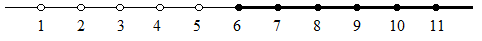
\includegraphics[width=4.46in,height=0.43in]{./media/image11.png}
	\end{Center}
\end{figure}


%%%%%%%%%%%%%%%%%%%% Figure/Image No: 11 Ends here %%%%%%%%%%%%%%%%%%%%

\par

b) \par


\vspace{\baselineskip}


%%%%%%%%%%%%%%%%%%%% Figure/Image No: 12 starts here %%%%%%%%%%%%%%%%%%%%

\begin{figure}[H]
	\begin{Center}
		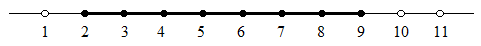
\includegraphics[width=4.4in,height=0.48in]{./media/image12.png}
	\end{Center}
\end{figure}


%%%%%%%%%%%%%%%%%%%% Figure/Image No: 12 Ends here %%%%%%%%%%%%%%%%%%%%

\par

c)\par



%%%%%%%%%%%%%%%%%%%% Figure/Image No: 13 starts here %%%%%%%%%%%%%%%%%%%%

\begin{figure}[H]
	\begin{Center}
		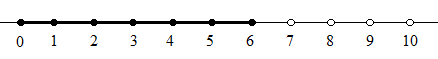
\includegraphics[width=4.56in,height=0.61in]{./media/image13.png}
	\end{Center}
\end{figure}


%%%%%%%%%%%%%%%%%%%% Figure/Image No: 13 Ends here %%%%%%%%%%%%%%%%%%%%

\par

d)\par



%%%%%%%%%%%%%%%%%%%% Figure/Image No: 14 starts here %%%%%%%%%%%%%%%%%%%%

\begin{figure}[H]
	\begin{Center}
		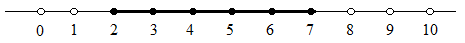
\includegraphics[width=4.84in,height=0.45in]{./media/image14.png}
	\end{Center}
\end{figure}


%%%%%%%%%%%%%%%%%%%% Figure/Image No: 14 Ends here %%%%%%%%%%%%%%%%%%%%

\par

e)\par



%%%%%%%%%%%%%%%%%%%% Figure/Image No: 15 starts here %%%%%%%%%%%%%%%%%%%%

\begin{figure}[H]
	\begin{Center}
		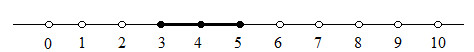
\includegraphics[width=4.94in,height=0.54in]{./media/image15.png}
	\end{Center}
\end{figure}


%%%%%%%%%%%%%%%%%%%% Figure/Image No: 15 Ends here %%%%%%%%%%%%%%%%%%%%

\par

f)\par



%%%%%%%%%%%%%%%%%%%% Figure/Image No: 16 starts here %%%%%%%%%%%%%%%%%%%%

\begin{figure}[H]
	\begin{Center}
		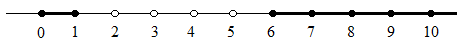
\includegraphics[width=4.83in,height=0.5in]{./media/image16.png}
	\end{Center}
\end{figure}


%%%%%%%%%%%%%%%%%%%% Figure/Image No: 16 Ends here %%%%%%%%%%%%%%%%%%%%

\par


\vspace{\baselineskip}
	\item a) Sim, b) Sim, c) Sim, mas em geral, é um número fracionário d) Sim e) Sim, mas em geral, é um número fracionário.\par

	\item Não\par

	\item Não existe\par

	\item a)Sim, b) Não, c) Sim e d) Não
\end{enumerate}\par


\vspace{\baselineskip}
\setlength{\parskip}{8.04pt}
\begin{adjustwidth}{0.3in}{0.0in}
\textbf{EXERCÍCIOS 3}\par

\end{adjustwidth}


\vspace{\baselineskip}
\setlength{\parskip}{9.96pt}
\begin{enumerate}
	\item  a) 3\ \ \ \  b) -25\ \  \  c) -9\ \ \ \  d) -1\ \ \ \ \  e) -2\ \ \ \  f) 35\ \ \ \ \  g) 0\ \  \  h) -22\  \   i) -8 \ \ \ \  j) 10\par

	\item R$\$$  -850,00\par

	\item a) 50 – 30 = 20\tab b) 100 – 40 = 60  \tab c) -100 + 50 = -50\tab d) -200 – 70 = -270\par

	\item + 21ºC\par

	\item – 10ºC \par

	\item 220m\par

	\item Sim, ( – 2)\par

	\item  \( 6/2=~3   \in Z;6/4 \notin  Z \)  
\end{enumerate}\par

\setlength{\parskip}{8.04pt}
\begin{adjustwidth}{0.3in}{0.0in}
\textbf{3.9 } \  a)\ 16\ \ \ \ \ b)\ -64\ \ \  c) 0     d)\ 1\ \   \ \  e)\ +25\ \ \ \ f)\ +16\ \ \ \ g) -16     h) -32\par

\end{adjustwidth}

\begin{adjustwidth}{0.3in}{0.0in}
\textbf{3.10  }a) $ \pm $ \ 3\ \ \ \ b)\ 3\ \ \ \ \ \ \ c)\ -3\ \ \ \ d)\ $ \pm $ \ 2\ \ \ \ e)\ $ \pm $ \ 2\ \ \ \  f) +2      g) -2       h) -4\par

\end{adjustwidth}


\vspace{\baselineskip}
\begin{adjustwidth}{0.3in}{0.0in}
\textbf{EXERCÍCIOS 4}\par

\end{adjustwidth}


\vspace{\baselineskip}
\setlength{\parskip}{9.96pt}
\begin{enumerate}
	\item a) -1\tab b) -11/10\ \ \  \tab c) ½\tab  d) 1 \ \ \ \ \ \  e) 1/24\tab f) 1\par


\vspace{\baselineskip}
\setlength{\parskip}{8.04pt}
\setlength{\parskip}{9.96pt}
	\item a) -1/2\tab b) 4/9\ \ \ \ \ \ \  c) -13/2\tab d)-1/5\ \ \ \ \ \ \  e) 30\tab f) 3/2
\end{enumerate}\par


\vspace{\baselineskip}
\setlength{\parskip}{8.04pt}
\begin{adjustwidth}{0.3in}{0.0in}
\textbf{EXERCÍCIOS 5}\par

\end{adjustwidth}


\vspace{\baselineskip}
\setlength{\parskip}{9.96pt}
\begin{enumerate}
	\item a) 3\tab b) 2/3\tab \tab c) 4\tab d) 2\tab e) 4\tab f) 5/3\par

	\item  Racionais\par

	\item a)  \( 2\sqrt[]{2} \) \tab b)  \( 2\sqrt[]{3} \) \ \ \  \tab c)  \( 2\sqrt[3]{3} \) \tab \tab d)  \( 2\sqrt[4]{2} \) \ \ \ \ \ \ \ \ \  e)  \( \frac{2\sqrt[]{3}}{3\sqrt[]{5}} \) \tab \tab f)  \( \frac{2\sqrt[3]{2}}{5} \) \par

	\item  Irracionais \par

	\item  a)  \( \sqrt[]{12} \) \tab b)  \( \sqrt[3]{54} \) \tab \tab c)  \( \sqrt[]{98} \) \tab \tab d) \( ~\sqrt[3]{\frac{1}{2}} \) \ \ \ \ \ \ \ \ \ \  e)  \( \sqrt[]{\frac{9}{2}} \) \ \ \ \ \ \ \ \  f)  \( \sqrt[]{\frac{75}{4}} \) \par

	\item a)  \( 7\sqrt[]{3} \) \tab b)  \( -2\sqrt[]{\frac{1}{2}} \)  \  \ \  c)  \( \sqrt[6]{500} \) \tab \ \ \  d)  \( \sqrt[]{\frac{15}{2}} \) \ \ \ \  e)  \( 3\sqrt[3]{\frac{3}{8}} \) \tab f)  \( 21\sqrt[]{10} \) \ \ \  g)  \( \sqrt[]{5} \) \tab h)  \( \sqrt[]{20} \) \par

	\item  a)  \( 8\sqrt[]{5} \) \tab b)  \( \sqrt[]{6}+\sqrt[]{10} \) \ \ \   c)  \( 8\sqrt[]{3}-3\sqrt[]{2} \) \tab d)  \( 2 \) \ \ \  \tab  e)  \( 14-6\sqrt[]{5} \) \tab \ \ \ \ \  f)  \( -5 \) \par


\vspace{\baselineskip}
\setlength{\parskip}{8.04pt}
\setlength{\parskip}{9.96pt}
	\item \  a)  \( \frac{\sqrt[]{3}}{3} \) \tab b)  \( \frac{3\sqrt[]{2}}{2} \) \ \  \  c)  \( \frac{7\sqrt[]{5}}{5} \) \ \ \ \ \  d)  \( 6-3\sqrt[]{3} \) \ \ \ \  e)  \( -\sqrt[]{2}-\sqrt[]{3} \) \tab f)  \( \frac{-175-35\sqrt[]{3}}{22} \) 
\end{enumerate}\par


\vspace{\baselineskip}
\setlength{\parskip}{8.04pt}
\begin{adjustwidth}{0.3in}{0.0in}
\textbf{5.9\  }São iguais.\par

\end{adjustwidth}

\begin{adjustwidth}{0.3in}{0.0in}
\textbf{5.10 }Respectivamente: \textbf{\textit{N, Z, Z, I, Q, N, Z, I, Q, Q, Q. }}\par

\end{adjustwidth}

\begin{adjustwidth}{0.3in}{0.0in}
\textbf{5.11} Porque o conjunto dos números Inteiros (Z) está contido no conjunto dos números Racionais (Q).\par

\end{adjustwidth}

\begin{adjustwidth}{0.3in}{0.0in}
\textbf{5.12}  -15\ é um número inteiro, mas também é racional, porque podemos escrevê-lo  na forma de fração: -30/2, por exemplo.\par

\end{adjustwidth}

\begin{adjustwidth}{0.3in}{0.0in}
\textbf{5.13} \  a)  \( \frac{3}{10} \) \tab  b)  \( \frac{5}{9} \) \ \ \ \ \ \   c)  \( \frac{132}{100} \) \tab d)  \( \frac{7}{33} \) \ \ \ \ \  \  e)  \( \frac{4}{3} \) \tab \tab f)  \( \frac{340}{99} \) \ \  \par

\end{adjustwidth}

\begin{adjustwidth}{0.3in}{0.0in}
\textbf{5.14\  }Porque é um número decimal periódico infinito.\par

\end{adjustwidth}

\begin{adjustwidth}{0.3in}{0.0in}
\textbf{5.15\  }Porque é um número decimal não periódico.\par

\end{adjustwidth}

\begin{adjustwidth}{0.3in}{0.0in}
\textbf{5.16\  }Devido\ à equivalência de frações, pois   \( \frac{2}{3} \cdot \frac{2}{2}=\frac{4}{6} \) . \par

\end{adjustwidth}

\begin{enumerate}[label*={\fontsize{12pt}{12pt}\selectfont \textbf{\textit{\arabic*.}}}]
	\item \  a)  \( Q \) \tab b)  \( Q \) \tab c)\textbf{\textit{  \( N \) \ \ \ \  }}d)\textbf{\textit{  \( Q \) }}\tab e)\textbf{\textit{  \( Q \) }}\tab f)\textbf{\textit{  \( Q \)  \tab }} g)\textbf{\textit{  \( Q \) \tab }}\ \  h)  \( Q \) \tab \ \ \ \ \  i) \( ~N \) \tab j)\textbf{\textit{  \( R \) }}\par

\setlength{\parskip}{9.96pt}
	\item \textbf{\textit{ }} a)  \( A =  \{ x N/ x < 6 \}  \) 
\end{enumerate}\par

\setlength{\parskip}{8.04pt}
\begin{adjustwidth}{0.3in}{0.0in}
\tab  b)  \( B =  \{ x Z/ -4 < x < 3 \}  \) \par

\end{adjustwidth}

\begin{adjustwidth}{0.3in}{0.0in}
\tab  c)  \( C =  \{ x~R\frac{}{}x~ -3 \}  \) \par

\end{adjustwidth}

\begin{adjustwidth}{0.3in}{0.0in}
\tab  d)  \( D =  \{ x  R / -3 < x < 5 \}  \) \par

\end{adjustwidth}

\begin{adjustwidth}{0.3in}{0.0in}
\tab  e)  \( E =  \{ x  R / 3 > x> 5 \}  \) \par

\end{adjustwidth}


\vspace{\baselineskip}
\begin{adjustwidth}{0.3in}{0.0in}
\textbf{5.19}\textit{ } a)\par

\end{adjustwidth}



%%%%%%%%%%%%%%%%%%%% Figure/Image No: 17 starts here %%%%%%%%%%%%%%%%%%%%

\begin{figure}[H]
	\begin{Center}
		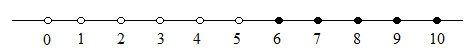
\includegraphics[width=3.92in,height=0.58in]{./media/image17.png}
	\end{Center}
\end{figure}


%%%%%%%%%%%%%%%%%%%% Figure/Image No: 17 Ends here %%%%%%%%%%%%%%%%%%%%

\setlength{\parskip}{9.96pt}
\par

\begin{adjustwidth}{0.3in}{0.0in}
 b)\par

\end{adjustwidth}



%%%%%%%%%%%%%%%%%%%% Figure/Image No: 18 starts here %%%%%%%%%%%%%%%%%%%%

\begin{figure}[H]
	\begin{Center}
		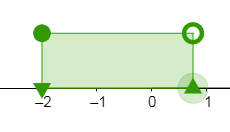
\includegraphics[width=3.83in,height=0.53in]{./media/image18.png}
	\end{Center}
\end{figure}


%%%%%%%%%%%%%%%%%%%% Figure/Image No: 18 Ends here %%%%%%%%%%%%%%%%%%%%

\par

\begin{adjustwidth}{0.3in}{0.0in}
 c)\par

\end{adjustwidth}



%%%%%%%%%%%%%%%%%%%% Figure/Image No: 19 starts here %%%%%%%%%%%%%%%%%%%%

\begin{figure}[H]
	\begin{Center}
		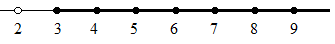
\includegraphics[width=3.49in,height=0.46in]{./media/image19.png}
	\end{Center}
\end{figure}


%%%%%%%%%%%%%%%%%%%% Figure/Image No: 19 Ends here %%%%%%%%%%%%%%%%%%%%

\par

\begin{adjustwidth}{0.3in}{0.0in}
 d)\par

\end{adjustwidth}



%%%%%%%%%%%%%%%%%%%% Figure/Image No: 20 starts here %%%%%%%%%%%%%%%%%%%%

\begin{figure}[H]
	\begin{Center}
		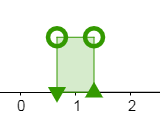
\includegraphics[width=4.17in,height=0.56in]{./media/image20.png}
	\end{Center}
\end{figure}


%%%%%%%%%%%%%%%%%%%% Figure/Image No: 20 Ends here %%%%%%%%%%%%%%%%%%%%

\par

\begin{adjustwidth}{0.3in}{0.0in}
 e)\par

\end{adjustwidth}



%%%%%%%%%%%%%%%%%%%% Figure/Image No: 21 starts here %%%%%%%%%%%%%%%%%%%%

\begin{figure}[H]
	\begin{Center}
		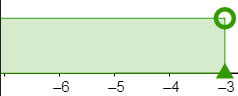
\includegraphics[width=4.38in,height=0.45in]{./media/image21.png}
	\end{Center}
\end{figure}


%%%%%%%%%%%%%%%%%%%% Figure/Image No: 21 Ends here %%%%%%%%%%%%%%%%%%%%

\par


\vspace{\baselineskip}
\begin{adjustwidth}{0.29in}{0.0in}
\textbf{5.20} O número representado por este produto notável é racional (16).\par

\end{adjustwidth}


\vspace{\baselineskip}
\setlength{\parskip}{8.04pt}

\vspace{\baselineskip}

\vspace{\baselineskip}

\vspace{\baselineskip}

\vspace{\baselineskip}
\setlength{\parskip}{6.0pt}

\printbibliography
\end{document}